\documentclass[a4paper]{article}
\usepackage{graphicx}
\usepackage{xcolor}
\usepackage{lineno}
\usepackage[brazil]{babel}
\usepackage[utf8]{inputenc}
\usepackage[T1]{fontenc}
\usepackage[autostyle]{csquotes}
\usepackage[colorinlistoftodos,portuguese,linecolor=black]{todonotes}
\usepackage{marginnote}
\usepackage{hyperref}
\usepackage[default,scale=0.95]{opensans}
\usepackage{fancyhdr}
\usepackage{pgf,tikz,pgfplots}
\usepackage{amsfonts}
\usepackage{amssymb}
\usepackage{mathtools}
\usepackage{mathrsfs}
\usepackage{nameref}
\usepackage{indentfirst}
\usepackage{array}
\usepackage{cancel}
\usepackage{enumitem}
\usepackage[most]{tcolorbox}
\usepackage[alf]{abntex2cite}

\setlength{\parskip}{\baselineskip}
%\setlength{\parindent}{0pt}%

\usetikzlibrary{arrows,chains,fit,quotes,positioning,shapes}
\pgfplotsset{compat=1.13}

% Set the overall layout of the tree
\tikzstyle{level 1}=[level distance=3.5cm, sibling distance=3.5cm]
\tikzstyle{level 2}=[level distance=3.5cm, sibling distance=2cm]

\newcommand{\aula}[2][]{\todo[inline,color=blue!10, #1]{\textbf{#2}}}
\newcommand{\nota}[2][]{\todo[color=yellow!30,linecolor=black, #1]{#2}}
\newcommand{\revisar}[2][]{\todo[color=red!30,linecolor=black, #1]{#2}}
\newcommand{\notagrande}[2][]{\todo[inline,color=orange!30, #1]{#2}}
\newcommand*\bolinha[1]{\tikz[baseline=(char.base)]{
		\node[shape=circle,draw,inner sep=2pt] (char) {#1};}}
\newcommand{\notaesq}[2][]{{%
		\let\marginpar\marginnote
		\reversemarginpar
		\renewcommand{\baselinestretch}{0.8}%
		\nota[#1]{#2}}}
\renewcommand\CancelColor{\color{red}}
\newcommand\defeq{\mathrel{\overset{\makebox[0pt]{\mbox{\normalfont\tiny\sffamily def}}}{=}}}
\newcommand\noteq{\mathrel{\overset{\makebox[0pt]{\mbox{\normalfont\tiny\sffamily not}}}{=}}}

\definecolor{ffqqqq}{rgb}{1.,0.,0.}
\definecolor{qqzzcc}{rgb}{0.,0.6,0.8}
\definecolor{eqeqeq}{rgb}{0.8784313725490196,0.8784313725490196,0.8784313725490196}

\fancypagestyle{plain}{
	\fancyhf{} %Clear Everything.
	\fancyfoot[C]{\thepage} %Page Number
	\renewcommand{\headrule}{\hrule height 2pt \vspace{1mm}\hrule height 1pt}
	\renewcommand{\footrulewidth}{1pt}
	\fancyfoot[L]{BOTTOM LEFT}
	\fancyfoot[R]{BOTTOM RIGHT}
	\fancyhead[LE]{TOP LEFT, EVEN PAGES}
	\fancyhead[RO]{TOP RIGHT, ODD PAGES}
}
\fancyfoot[C]{\sffamily\textbf{\thepage}}

\renewcommand\seriesdefault{l}
\renewcommand\mddefault{l}
\renewcommand\bfdefault{sb}

\hypersetup{
	colorlinks  = true,
	allcolors   = black,
	pdftitle    = {Caderno de IPE},
	pdfsubject  = {Estatística},
	pdfauthor   = {Caio César Carvalho Ortega},
	pdfcreator  = {Caio César Carvalho Ortega},
	pdfproducer = {Caio César Carvalho Ortega},
	pdfkeywords = {estatística, probabilidade}
}

\definecolor{CinzaCaixa}{gray}{0.85}
\newtcolorbox{citacao}{colback=CinzaCaixa,grow to right by=-10mm,grow to left by=-10mm,
	boxrule=0pt,boxsep=0pt,breakable}

\SetBlockEnvironment{citacao}

\definecolor{Red}{rgb}{0.9,0.0,0.1}
%\definecolor{Blue}{rgb}{0.1,0.1,0.9}
%\hyphenation{}
\pagestyle{fancy}

% ----------------------------------------------------------

\begin{document}
	
	\section{Prólogo}
	
	As anotações e considerações que se seguem foram realizadas de maneira autônoma e não são fruto de orientação por parte da universidade e/ou de qualquer membro do corpo docente. Foram realizadas para fins de estudo, sendo, portanto, reflexo de um esforço de cunho pessoal para melhor apreensão do conteúdo discutido em sala.
	
%	\nocite{ross2010}
%	\nocite{morin2016}
%	\nocite{lipson2011}

	\aula{Início da aula de 25/06/2019}
	
	\section{Introdução à Estatística Descritiva}
	
	Conteúdo proposto:
	
	\begin{itemize}
		\item Conceitos básicos
		\begin{itemize}
			\item Elemento
			\item Dado e variável
			\item Valor e conjunto de valores
			\item Tipo de dado e tipo de variável
		\end{itemize}
		\item Tabelas
		\begin{itemize}
			\item Frequência
		\end{itemize}
		\item Gráficos
		\begin{itemize}
			\item Variável qualitativa
			\item Variável quantitativa
		\end{itemize}
	\end{itemize}
	
	A coisa mais importante na Estatística são os dados, designados como elementos, que podem ser muita coisa, uma entidade, um sujeito, uma pessoa, uma observação, um experimento. Por exemplo: o professor nasceu em Avaré, eis um dado; dizer que o céu desta noite está estrelado é uma observação, ou seja, um dado que veio de uma observação; já a ideia do experimento é ser um dado fruto de um processo controlado, como uma receita de bolo. Tudo isso são dados.
	
	O dado é um fato, uma característica, de um elemento. Nacionalidade, gentílico, cidade-natal, avaliação do bolo produzido com a receita (se ficou gostoso ou não).
	
	Valor é um agrupamento de dados, ou ainda, valores que os dados poderão ter. Podemos falar também em conjunto de valores.
	
	Quanto ao tipo de dado ou variável, estes podem ser qualitativos (também chamados de categorizados) e quantitativos. Qualitativa: todos aqueles dados e variáveis que não são números (exemplo: local de nascimento), subdivididos em nominal (exemplo: bolo gostoso ou bolo ruim) e ordinal (exemplo: altura de uma pessoa); uma variável qualitativa pode ser uma variável discreta (que só pode assumir valores inteiros) ou contínua (que pode assumir qualquer valor, podendo ser decimal).
	
	Tomando por base o exercício 2 do arquivo ``apostila completa.pdf'', Munhoz começa a responder cada uma das questões.
	
	\begin{enumerate}[label=\alph*.]
		\item 6
		\item 4
		\item 24
		\item Qualitativa: gênero\\ Quantitativa: idade, questão do aborto, classificação
		\item Não
	\end{enumerate}
	
	Feito o exercício, devemos compreender os conceitos de (i) frequência absoluta, que pode ser definido como: quantidade de ocorrência de um valor ou conjunto de valores; (ii) tabela de frequência absoluta, que pode ser definida como a tabela em que as linhas expressam as frequências de cada valor ou conjunto de valores.
	
	Munhoz agora parte para o exercício 8D no mesmo arquivo PDF. Professor inicia a construção de uma tabela de frequências absolutas. Em seguida, complementa com a coluna de frequências relativas. Vide \autoref{tab:tab1}.
	
	\begin{table}[h]
		\centering
		\caption{Opinião dos funcionários sobre troca de gerente (G = gosta; N = não gosta)}
		\begin{tabular}{|l|l|l|}
			\hline
			\textbf{Opinião} & \textbf{Frequência absoluta} & \textbf{Frequência relativa} \\ \hline
			G & 9 & 45\% \\ \hline
			N & 11 & 55\% \\ \hline
		\end{tabular}
		\\ \vspace{1mm} Fonte: questão 8
		\label{tab:tab1}
	\end{table}
	
	Tabelas possuem título, corpo e fonte.
	
	Frequência relativa é o percentual do aparecimento de cada valor.
	
	Professor agora parte para o gráfico, dizendo que este torna a visualização mais fácil. Aponta que o gráfico pode ser de coluna ou de setores (também chamado de ``gráfico de pizza'').
	
	Desenha um gráfico de colunas e um gráfico de setores.
	
	Munhoz sugere a utilização do histograma para gráficos de variáveis quantitativas. O histograma também é conhecido como damo-e-folhas (vide \autoref{fig:damofolhas1}). Define-o como gráfico de colunas em faixas justapostas.
	
	\begin{figure}[]
		\centering
		\caption{Damo-e-folhas para a pontuação}
		\begin{tabular}{l|lllll}
			2 & 8 & 6 &  &  &  \\
			3 & 5 &  &  &  &  \\
			2 & 6 & 9 & 5 & 4 &  \\
			6 & 4 & 8 & 0 &  &  \\
			9 & 2 & 5 & 2 & 0 & 9
		\end{tabular}
		\\ \vspace{1mm} Fonte: questão 10E
		\label{fig:damofolhas1}
	\end{figure}
	
	Para permitir a construção do histograma, agrupa as pontuações em classes (vide \autoref{tab:pontuacaoalunos}).
	
	\begin{table}[h]
		\centering
		\caption{Pontuação dos alunos}
		\begin{tabular}{l|l|l|l}
			\textbf{Pontuação} & \textbf{Freq. absoluta} & \textbf{Freq. acum.} & \textbf{Freq. acum. (percent.)} \\ \hline
			50-59 & 3 & 3 & 15\% \\
			60-59 & 2 & 5 & 25\% \\
			70-79 & 5 & 10 & 50\% \\
			80-89 & 4 & 14 & 70\% \\
			90-99 & 6 & 20 & 100\%
		\end{tabular}
		\\ \vspace{1mm} Fonte: questão 10E
		\label{tab:pontuacaoalunos}
	\end{table}
	
	\subsection{Teste no Tidia}
	
	Questões 2c, 4e, 7 frequência absoluta de A e 11 frequência acumulada percentual da sexta classe da segunda lista, cada uma correspondendo às questões 1 a 4 do teste na plataforma, respectivamente.
	
	\aula{Início da aula de 28/06/2019}
	
	\section{Medidas de posição e variabilidade}
	
	\subsection{Medida de posição média para dados brutos}
	
	$X_{1}, X_{2}, X_{3}$
	
	Média = $M = \dfrac{X_{1} + X_{2} + \dots + X_{n}}{n}$
	
	\subsubsection{Exemplo}
	
	Vide gastos na \autoref{tab:gastomes}.
	
	\begin{table}[h]
		\centering
		\caption{Gasto por mês}
		\begin{tabular}{l|l}
			\textbf{Mês} & \textbf{Gasto} \\ \hline
			Janeiro & 200 \\
			Fevereiro & 500 \\
			Março & 600
		\end{tabular}
		\label{tab:gastomes}
	\end{table}
	
	O gasto médio então é expresso por:
	
	$M = \dfrac{200+500+600}{3} = \dfrac{1300}{3} \cong 433$
	
	\subsubsection{Notação}
	
	$M$ é a média populacional e $\bar{x}$ é a média de uma amostra; $f$ é a frequência absoluta.
	
	\subsection{Medida de posição média para dados agrupados}
	
	\notagrande{Passar a limpo da foto.}
	
	\subsection{Dados agrupados por faixas de valores}
	
	Troca a faixa pelo ponto central (o ponto médio) e calcula a média. Veja o exemplo da \autoref{tab:agrup6e}.
	
	\begin{table}[h]
		\centering
		\caption{Pontuação dos alunos}
		\begin{tabular}{l|l|l|l|l}
			\textbf{Chave} & \textbf{X} & \textbf{fa} & \textbf{f} & \textbf{fX} \\ \hline
			2-6 & 4 & 2 & 20\% & 0,8 \\
			7-11 & 9 & 3 & 30\% & 2,7 \\
			12-16 & 14 & 4 & 40\% & 5,6 \\
			17-21 & 19 & 1 & 10\% & 1,9 \\ \hline
			- & - & 10 & 11
		\end{tabular}
		\\ \vspace{1mm} Fonte: questão 6E
		\label{tab:agrup6e}
	\end{table}
	
	Logo a média é $11$ ($M=11$).
	
	\section{Média da variabilidade}
	
	\subsection{Desvio quadrático}
	
	Desvio quadrático é a diferença do quadrado do valor:
	
	\begin{equation*}
		\left( X_{i} -M \right)^{2}
	\end{equation*}
	
	Considerando novamente os gastos na \autoref{tab:gastomes} e que $M = 430$, temos:
	
	Desvio quadrático do $500$.
	
	\notagrande{Não deu tempo de copiar}
	
	Calculemos para os gastos dos exemplos anteriores (\autoref{tab:gastomesxi}).
	
	\begin{table}[h]
		\centering
		\caption{Gasto por mês}
		\begin{tabular}{l|l}
			\textbf{Valor} & \textbf{$(X_{i}-M)^{2}$} \\ \hline
			200 & 52900 \\
			500 & 4900 \\
			600 & 28900 \\ \hline
			- & 86700
		\end{tabular}
		\label{tab:gastomesxi}
	\end{table}
	
	\subsection{Variância}
	
	Variância é a média dos desvios quadráticos, expressa com o símbolo $\sigma^{2}$ (sigma ao quadrado). Para a variância dos dados $X{1}, X_{2}, \dots, X_{n}$ com média $M$:
	
	\begin{equation*}
		\sigma{2} = \dfrac{(X_{1} + M)^{2} + (X_{2}  + M)^{2} + \dots + (X_{n} - M)^{2} }{n}
	\end{equation*}
	
	Adotemos novamente os gastos dos exemplos anteriores para cálculo da variância:
	
	$\sigma^{2} = \dfrac{52900 + 4900 + 28900}{3} = \dfrac{86700}{3} = 28900$
	
	\subsection{Coeficiente de variação}
	
	É o $CV$. A notação é $CV = \dfrac{\sigma}{M}$. Exemplo:
	
	$CV = \dfrac{170}{430} = 39\%$
	
	\section{Variância para dados brutos}
	
	Sendo $f =$ frequência relativa, temos a \autoref{tab:vdb}.
	
	\begin{table}[h]
		\centering
		\caption{Tabela para exemplificar variância para dados brutos}
		\begin{tabular}{l|l|l|l|l}
			\textbf{$X$} & \textbf{$f$} & \textbf{$fX$} & \textbf{$(X_{i} - M)^{2}$} & \textbf{$f(X_{i}-M)^{2}$} \\ \hline
			$X_{1}$ & $f_{1}$ & $f_{1}X_{1}$ & $(X_{1} - M)^{2}$ & $f_{1}(X_{1}-M)^{2}$ \\
			$X_{1}$ & $f_{1}$ & $f_{1}X_{1}$ & $(X_{1} - M)^{2}$ & $f_{1}(X_{1}-M)^{2}$ \\
			$X_{1}$ & $f_{1}$ & $f_{1}X_{1}$ & $(X_{1} - M)^{2}$ & $f_{1}(X_{1}-M)^{2}$ \\ \hline
			- & - & $M$ & - & $\sigma{2}$
		\end{tabular}
		\label{tab:vdb}
	\end{table}
	
	\subsection{Variância populacional e desvio populacional}

	\notagrande{Passar a limpo da foto.}
	
	\subsection{Percentis}
	
	É uma medida de posição. Sendo o percentil um ponto entre $p\%$ e $(-1p)\%$, temos:
	
	\begin{equation*}
		p = \underbracket{p \times n}_{\text{arredondado pra cima}}
	\end{equation*}
	
	$n$ é a quantidade de dados.
	
	Exemplo a partir da questão 3A, alínea (d):
	
	$p_{75}$ está na posição $75\% \times 8 = 6$
	
	O ranking é expresso pelos dados ordenados como \bolinha{30} \bolinha{36} \bolinha{42} \bolinha{42} \bolinha{44}
	\bolinha{46} \bolinha{50} \bolinha{54}
	
	Então $p_{75} = \dfrac{46+50}{2} = 48$
	
	$p_{75} = 48 = Q_{3}$ (3o. quartil)
	
	$p_{25} = Q_{1}$ (1o. quartil)
	
	$p_{25} = \dfrac{36 + 42}{2} = 39$
	
	$p_{50} = Q_{2} =$ mediana  $=\dfrac{42 + 44}{2} = 43$
	
	\notagrande{Box-plot na foto. Passar a limpo}
	
	Exemplo respondendo a questão 9C:
	
	$CV_{UTC} = \dfrac{0,84}{2,8} = 30\%$
	
	$CV_{UTK} = \dfrac{0,84}{2,4} = 37\%$
	
	Logo, a UTK tem notas mais dispersas.
	
	\notagrande{A P1 ficou para dia 19/7!}
	
	Responder no Tidia:
	
	\begin{enumerate}
		\item 3 (a + c + d)
		\item 7 (a + b)
		\item 10 (cidade e dispersão)
		\item 17 resposta: 131
	\end{enumerate}

	\aula{Início da aula de 05/07/2019}

	% Apostila 4

	\section{Probabilidade: contextos básicos}

	\begin{itemize}
		\item Ementa:
		\begin{itemize}
			\item Probabilidade
			\item Probabilidade da ação
			\item Probabilidade condicional
		\end{itemize}
	\end{itemize}

	\subsection{Definições}
	
	\textbf{Evento}: conjunto de resultados.
	
	\textbf{Espaço amostral}: conjunto de todos os resultados possíveis
	
	\textbf{Ponto amostral}: é um elemento do espaço amostral
	
	\subsection{Exemplo}
	
	\noindent Dado o lançamento de uma moeda, são:
	
	$A =$ espaço amostral
	
	$A = \{cara,coroa\}$
	
	Pontos amostrais: cara, coroa
	
	\subsection{Exemplo}
	
	\noindent Dado o lançamento de duas moedas, são:
	
	$A =$ espaço amostral
	
	$A = \{(cara,coroa),(coroa,cara),(cara,cara),(coroa,coroa)\}$
	
	Pontos amostrais: (cara,coroa), (coroa,cara), (cara,cara), (coroa,coroa)
	
	$E =$ é o evento, no caso, \textbf{sair uma cara somente}
	
	$E = \{(cara,coroa),(coroa,cara)\} \subset A$
	
	\subsection{Definição de probabilidade}
	
	$P(E) =$ probabilidade do evento $E$
	
	$E \subset A, A = $espaço amostral
	
	$P(E) = \dfrac{n(E)}{n(A)} = \dfrac{\text{quantidade de elementos de $E$}}{\text{quantidade de elementos de $A$}}$
	
	\subsection{Exemplo}
	
	Considere o seguinte experimento: lançamento de uma moeda. Temos:
	
	$A = \{cara,coroa\}$
	
	$E =$ sair cara
	
	$E = \{(cara)\}$
	
	$P(E) = P(cara) = \dfrac{n(E)}{n(A)} = \dfrac{1}{2} = 50\%$
	
	\subsection{Exemplo}
	
	Considere o seguinte experimento: lançamento de duas moedas. Temos:
	
	$E =$ sair só uma cara
	
	$P(E) = \dfrac{2}{4} = \dfrac{1}{2} = 50\%$
	
	\subsection{Definição frequentista de probabilidade}
	
	Nela, a probabilidade ($P$) é igual a frequência relativa. Por exemplo, lançar uma moeda e esperar $500$ caras. Segundo \citeonline[p, 121]{bussab2002}, esta ``se baseia na estabilidade das freqüências relativas e no fato
	de podermos, hipoteticamente, repetir um experimento várias vezes''.
	
	\subsection{Exemplo}
	
	\noindent Referência: 3A, apostila 4
	
	\begin{enumerate}[label=\alph*.]
		\item $\{0,1,2,3,4\}$ \\ $5$
		\item $0$, cujo $P = 60 \div 200 = 30\%$ \\
			$1$, cujo $P = 80 \div 200 = 40\%$ \\ 
			$2$, cujo $P = 40 \div 200 = 20\%$ \\
			$3$, cujo $P = 16 \div 200 = 8\%$ \\
			$4$, cujo $P = 4 \div 200 = 2\%$
		\item $P(V=0) = 30\%$
		\item $P(V \geq 2) = 20\% + 8\% + 2\% = 30\%$
		\item $P(V=1$ ou $V=2) = 40\% + 20\% = 60\%$ ou, alternativamente \\
			$P(V=1$ ou $V=2) = \dfrac{120}{200} = 60\%$
		\item $P(V=2$ ou $V=1$ ou $V=0) = \dfrac{180}{200} = 90\%$ ou, alternativamente \\
			$P(V2$ ou $V=1$ ou $V=0) = 20\% + 40\% + 30\% - 90\%$
	\end{enumerate}
	
	\subsection{Probabilidade da união}
	
	\subsubsection{Proposição}
	
	Proposição: $P(A \cup B) = P(A) + P(B) - P(A \cap B)$
	
	Prova: $n =$ quantidade total de possibilidades $=$ tamanho do espaço amostral.
	
	Temos:
	
	$n_A\cup B = n_A + n_B - n_{A \cap B}$
	
	$\dfrac{n_{A\cup B}}{n} = \dfrac{n_{A}}{n} + \dfrac{n_B}{n} - \dfrac{n_{A \cap B}}{n}$

	Logo:
	
	$P(A \cup B) = P(A) + P(B) - P(A \cap B)$
	
	\subsubsection{Exemplo}
	
	Professor utiliza o exemplo $n_{B \cup C} = n_{B} + n_{C} - n_{B \cap C}$, vide \autoref{fig:exemplo2conj}.
	
	\begin{figure}[h]
		\centering
		\caption{Observar interseção}
		\begin{tikzpicture}[
		thick]
		\draw [fill=cyan, fill opacity=0.5] (0,0) circle (2cm);
		\draw [fill=orange, fill opacity=0.5] (3,-1) circle (2.5cm);
		\draw (0,0) ++(120:2cm) -- ++(120:2.2cm) node [fill=white,inner sep=5pt](a){$B$};
		\draw (3, -1) ++(30:2.5cm) -- ++(30:2.6cm) node [fill=white,inner sep=5pt](b){$C$};
		\end{tikzpicture}
		\label{fig:exemplo2conj}
	\end{figure}
	
	\subsubsection{Definição}
	
	$A$ e $B$ são eventos excludentes \hspace{5mm} $\leftrightarrow A \cap B = \emptyset$
	
	\subsubsection{Proposição}
	
	$A$ e $B$ são eventos excludentes \hspace{5mm} $\leftrightarrow P(A \cup B) = P(A) + P(B)$
	
	\subsubsection{Exemplo}
	
	Referência: exercício 1A da apostila 4
	
	$P(A) = 23\%$
	
	$P(A) = 19\%$
	
	$P(A$ ou $B) = P(A \cup B) = 38\%$
	
	\begin{enumerate}[label=\alph*.]
		\item $P(A \cap B) = ?$ \\
			\\
			Temos: \\
			\\
			$P(A \cup B) = P(A) + P(B) - P(A \cap B)$ \\
			$P(A \cap) B) = P(A) + P(B) - P(A \cup B)$ \\
			$P(A \cap) B) = 23\% + 19\% - 36\% = 42\% - 38\%$ \\
			$P(A \cap) B) =	4\%$
		\item Não são eventos excludentes, pois $A \cap B \neq \emptyset$ devido a $P(A \cap B) > 0$
	\end{enumerate}

	\subsection{Probabilidade condicional}
	
	\subsubsection{Definição}
	
	\begin{equation*}
		P(A | B) = \dfrac{N_{A \cap B}}{N_B}
	\end{equation*}
	
	\begin{displaycquote}[p. 75]{pinheiro2009}
		Se A e B são eventos que podem ocorrer em um dado experimento, a probabilidade condicional de $B$ ter ocorrido, quando se sabe que $A$ ocorreu, é representada por $P(B|A)$. (Leia-se probabilidade de $B$ dado $A$)
	\end{displaycquote}
	
	\subsubsection{Exemplo}
	
	Considere a retirada de bolas pretas e brancas numa caixa:
	
	\bolinha{P} \bolinha{P} \bolinha{P} \bolinha{B} \bolinha{B}
	
	$P(\text{sair bola preta na 2a. vez }|\text{ sair bola branca na 1a. vez}) = \dfrac{3}{4} = 75\%$

	$P(\text{sair bola preta na 2a. vez }|\text{ sair bola branca na 1a. vez}) = \dfrac{2}{4} = 50\%$	
	
	Experimento 1: tira uma bola
	
	Experimento 2: tira uma bola
	
	\bolinha{P} \bolinha{P} \bolinha{P} \bolinha{B} \bolinha{B} $\rightarrow$ 1a. vez $\rightarrow$ \bolinha{P} \bolinha{P} \bolinha{B} \bolinha{B} $\rightarrow$ 2a. vez

	\subsubsection{Exemplo}
	
	$A = \{1,2,3,4,5\}$
	
	$B = \{1,2\}$
	
	$C = \{7,8,9\}$
	
	\subsubsection{Proposição}
	
	$P(A|B) = \dfrac{P(A \cap B)}{P(B)}$
	
	\subsubsection{Prova}
	
	$P(A|B) = \dfrac{n_{A \cap B}}{n_B}$
	
	$P(A|B) = \dfrac{\frac{n_{A \cap B}}{n}}{\frac{n_B}{n}} = \dfrac{P(A \cap B)}{P(B)}$
	
	\subsubsection{Consequência}
	
	$P(A \cap B) = P(A|B) \cdot P(B)$
	
	\subsubsection{Definição}
	
	Eventos $A$ e $B$ são independentes \hspace{5mm} $\leftrightarrow P(A|B) = P(A)$
	
	\subsubsection{Proposição}
	
	$A$ e $B$ são eventos independentes \hspace{5mm} $\leftrightarrow P(A \cap B) = P(A) \cdot P(B)$
	
	\subsubsection{Prova}
	
	$P(A \cap B) = P(A|B)P(B) = P(A)P(B)$
	
	\subsubsection{Exemplo}
	
	Referência: exercício 8B da apostila 4
	
	\begin{enumerate}[label=\alph*.]
		\item $P(\text{cliente mulher}) = \dfrac{30 + 50}{200} = \dfrac{80}{200} = 40\%$
		\item $P(\text{cliente homem}) = \dfrac{100}{200} = 50\%$
		\item $P(\text{solteira }|\text{ mulher}) = \dfrac{30}{80} = 37,5\%$
		\item $\dfrac{12\cancel{0}}{20\cancel{0}} = 60\%$
		\item $P(\text{casado }|\text{ homem}) = \dfrac{100}{120} = 83,3\%$
		\item Não são, pois são iguais
		\item $P(\text{solteira }|\text{ mulher}) = \dfrac{30}{80} = 37,5\%$ \\
			$P(\text{solteiro}) = \dfrac{50}{200} = 25\%$\\
	\end{enumerate}

	\subsection{Teste no Tidia}
	
	Relação entre questão do Tidia e questão da apostila 4:
	
	\begin{enumerate}
		\item 7C. Resposta: $50\%$
		\item 9D. Resposta: $49\%$
		\item 11C. Resposta: $50\%$
		\item 10, considerando: \\
			$x+y$ \\
			$x = P(A \cap B) - P(A) \cdot P(B)$ \\
			$y = P(A \cup B) - P(A) - P(B)$
	\end{enumerate}
	
	\aula{Início da aula de 12/07/2019}
	
	% Apostila 5
	
	Faltei, mas sei que o Munhoz avançou mais uma apostila.
	
	Ementa:
	
	\begin{itemize}
		\item Diagrama de árvore
		\item Probabilidade do caminho
		\item Probabilidade inversa
		\item Teorema de Bayes
	\end{itemize}
	
	\section{Teorema de Bayes}
	
	Uma das relações mais importantes envolvendo probabilidades condicionais \citeonline[p. 116]{bussab2002}. Fórmula da versão mais simples \cite[p. 116]{bussab2002}:
	
	\begin{equation*}
		P(A|B) = \dfrac{P(A \cap B)}{P(B)} = \dfrac{P(A) \cdot P(B|A)}{P(B)}
	\end{equation*}
	
	Segundo \citeonline[p. 119]{bussab2002}, ``o Teorema de Bayes fornece um mecanismo formal para atualizar probabilidades'', além disso, possui ainda especial importância:
	
	\begin{displaycquote}[p. 119]{bussab2002}
		O Teorema de Bayes, que aparentemente poderia ser encarado como mais um resultado na teoria de probabilidades, tem importância fundamental, pois fornece a base para uma abordagem da inferência estatística conhecida como \textit{inferência bayesiana}.
	\end{displaycquote}

	\subsection{Exemplo}\label{sec:exbayes}
	
	\begin{displaycquote}[p. 118]{bussab2002}
		Para selecionar seus funcionários, uma empresa oferece aos candidatos um curso de treinamento durante uma semana. No final do curso, eles são submetidos a uma prova e 25\% são classificados como bons (B), 50\% como médios (M) e os restantes 25\% como fracos (F). Para facilitar a seleção, a empresa pretende substituir o treinamento por um teste contendo questões referentes a conhecimentos gerais e específicos. Para isso, gostaria de conhecer qual a probabilidade de um indivíduo aprovado no teste ser considerado fraco, caso fizesse o curso. Assim, neste ano, antes do início do curso, os candidatos foram submetidos ao teste e receberam o conceito aprovado (A) ou reprovado (R). No final do curso, obtiveram-se as seguintes probabilidades condicionais:
		
		\begin{equation*}
		P(A|B) = 0,80 \hspace{5mm} P(A|M) = 0,50 \hspace{5mm} P(A|F) = 0,20
		\end{equation*}
		
		Queremos encontrar $P(F | A)$ e, pelo Teorema de Bayes, essa probabilidade é dada por
		
		\begin{equation*}
			P(F|A) = \dfrac{P(A|F)P(F)}{P(A|B)P(B) + P(A|M)P(M) + P(A|F)P(F)}
		\end{equation*}
		
		\begin{equation*}
			= \dfrac{(0,20)(0,25)}{(0,80)(0,25)+(0,50)(0,50)+(0,20)(0,25)} = 0,10
		\end{equation*}
		
		Então, apenas 10\% dos aprovados é que seriam classificados como fracos durante o
		curso. De modo análogo podemos encontrar $P(B | A) = 0,40$ e $P(M | A) = 0,50$, que poderiam fornecer subsídios para ajudar na decisão de substituir o treinamento pelo teste.
	\end{displaycquote}

	\subsection{Diagrama em árvore}
	
	Auxiliar para solucionar  problemas envolvendo o Teorema de Bayes, como aquele observado na \autoref{sec:exbayes}.
	
	\begin{figure}
		\centering
		\caption{Diagrama em árvore para o exemplo da \autoref{sec:exbayes}}
		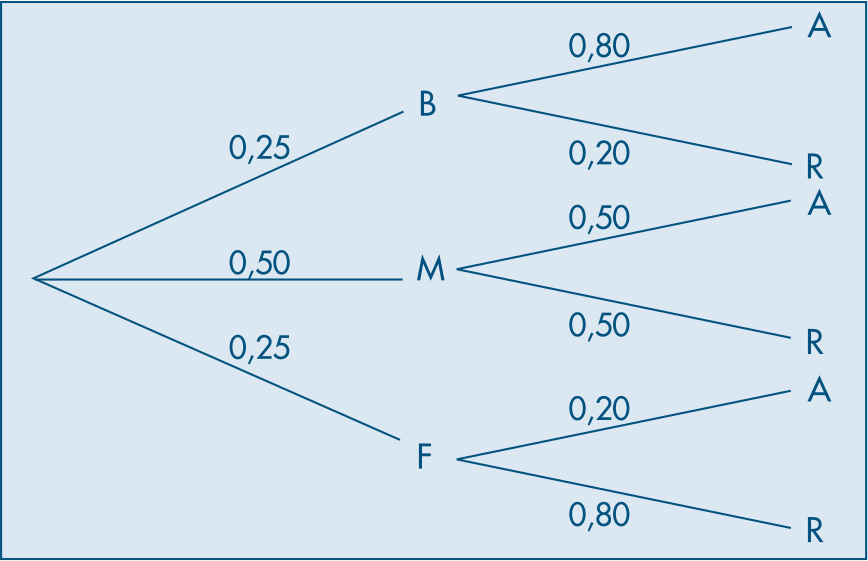
\includegraphics[width=0.7\linewidth]{img/diagrama_bayes}
		\\ \vspace{1mm} Fonte: \citeonline[p. 119]{bussab2002}
		\label{fig:diagramabayes}
	\end{figure}
	
	\subsection{Teste no Tidia}
	
	Relação entre questão do Tidia e questão da apostila 5.
	
	\begin{enumerate}
		\item 1A. Resposta: $35\%$
		\item 2F. Resposta: $25,75\%$
		\item 3. Resposta: $81,25\%$
		\item 6A. Resposta: $56,25\%$
	\end{enumerate}

	\aula{Início da aula de 23/07/2019}

	\section{Contagem e Probabilidade}
	
	Ementa:
	
	\begin{itemize}
		\item Objetivo
		\item Problema modelo
		\item Princípio fundamental da contagem
	\end{itemize}

	\subsection{Objetivo}
	
	Contar todas as possibilidades de uma situação sem listá-las.
	
	\subsection{Problema modelo}
	
	\noindent Uma cidade tem $n$ pontos turísticos e pretendo visitar $r$ destes, $r \leq n$.
	
	Quantidade de possibilidades de visitar todos numa certa ordem é $P_n =$ permutação de $n$ elementos.
	
	Quantidade de possibilidades de visitar $r$ pontos turísticos numa certa ordem é $A_{n,r} =$ arranjo de $n$ elementos tomados $r$ a $r$.
	
	Quantidade de possibilidades de visitar $r$ pontos sem levar em conta a ordem é $Cn,r =$ combinação de $n$ elementos tomados $r$ a $r$.
	
	\subsection{Problema}
	
	Pontos turísticos: $A, B, C$
	
	Visitar todos numa certa ordem tem as possibilidades: $ABC, ACB, BAC, BCA, CAB, CBA$, ou seja, a quantidade de permutações dos três elementos é seis, ao que temos: $P_3 = 6$.
	
	\subsection{Problema}
	
	Visitar $2$ pontos turísticos numa certa ordem tem as possibilidades: $AB, BA, AC, CA, BC, CB$, logo, $A_{3,2} = 6$.
	
	\subsection{Problema}
	
	Visitar $2$ pontos turísticos sem levar em conta a ordem, tem as possibilidades $\{A,B\}, \{A,C\}, \{B,C\}$. Perceba que as combinações são subconjuntos com $r$ elementos, logo $C_{3,2} = 3$.
	
	\subsection{Soluções}
	
	\subsubsection{Definição}
	
	Fatorial de $n$:
	
	\begin{equation*}
		n! = n \cdot (n-1) \cdot (n-2) \cdot \dots \cdot 2 \cdot 1
	\end{equation*}
	
	Exemplo: $5! = 5 \cdot 4 \cdot 3 \cdot 2 \cdot 1 = 120$
	
	$5! = 5 \cdot 4!$
	
	$5! = 5 \cdot 4 \cdot 3!$
	
	\subsubsection{Proposição}
	
	$P_n = n!$
	
	$A_{n,r} = \dfrac{n!}{(n-r)!}$
	
	$C_{n,r} = \dfrac{n!}{(n-r)! r!}$
	
	\subsubsection{Exemplo com arranjo}
	
	Vistos $4$ pontos turísticos de $11$, definindo o roteiro pode ser feito de:
	
	$A_{11,4} = \dfrac{11!}{(11-4)!}$
	
	$A_{11,4} = \dfrac{11!}{7!} = \dfrac{11 \cdot 10 \cdot 9 \cdot 8 \cdot \cancel{7!}}{\cancel{7!}} = 7920$ maneiras.
	
	\subsubsection{Exemplo com combinação}
	
	Visitar $4$ de $11$ pontos turísticos pode ser feito de:
	
	$C_{11,4} = \dfrac{11!}{(11-4)! 4!} = \dfrac{7920}{24} = 330$ maneiras.
	
	\subsubsection{Exemplo com permutação}
	
	Visitar todos os pontos turísticos definindo o roteiro pode ser feito de:
	
	$P_{11} = 11! = 11 \cdot 10 \cdot 9 \cdot \dots \cdot 1 = 39.916.800$ maneiras.
	
	\subsection{Princípio fundamental da contagem}
	
	Um conjunto $A$ tem $m$ elementos. Um conjunto $B$ tem $n$ elementos. A quantidade de elementos de $A \times B$ é $m \cdot n$.
	
	\notagrande{O $A$ no parágrafo anterior deve ser lido como ``A cartesiano B''}
	
	$m=5$ e $n=3$
	
	\begin{table}[h]
		\centering
		\caption{Representação dos pares ordenados}
		\label{tab:paresordenados}
		\begin{tabular}{llllll}
			$B_3$ & $\blacksquare$ & $\blacksquare$ & $\blacksquare$ & $\blacksquare$ & $\blacksquare$ \\
			$B_2$ & $\blacksquare$ & $\blacksquare$ & $\blacksquare$ & $\blacksquare$ & $\blacksquare$ \\
			$B_1$ & $\blacksquare$ & $\blacksquare$ & $\blacksquare$ & $\blacksquare$ & $\blacksquare$ \\
			& $A_1$ & $A_2$ & $A_3$ & $A_4$ & $A_5$
		\end{tabular}
	\end{table}
	
	$5 \cdot 3 = 15$ pares ordenados, vide \autoref{tab:paresordenados}.
	
	Um conjunto $A$ tem $m$ elementos. Um conjunto $B$ tem $n$ elementos. Um conjunto $C$ tem $p$ elementos.
	
	A quantidade de elementos $A \times B \times C$ (elementos = trios).
	
	\begin{equation*}
		m \cdot n \cdot p
	\end{equation*}
	
	\subsubsection{Exemplo com combinação}
	
	Contratar 4 pessoas num grupo de 10 candidatos.
	
	$C_{10,4} = \dfrac{10!}{6! 4!}$
	
	$= \dfrac{10 \cdot 9\cdot 8\cdot 7\cdot \cancel{6!}}{\cancel{6!} 4!}$
	
	$= \dfrac{5040}{24} = 210$
	
	\subsubsection{Exemplo com permutação}
	
	Uma casa tem $7$ portas. De quantas formas você pode entrar e sair da casa?
	
	$7 \cdot 7 = 49$
	
	\subsubsection{Exemplo}
	
	Quantos números de $4$ algarismos posso fazer com os algarismos $1,2,3,4,5,6,7,8,9$?
	
	Caso 1: sem restrição:
	
	$9 \cdot 9 \cdot 9 \cdot 9 = 6561$
	
	Caso 2: todos distintos:
	
	\bolinha{9} \bolinha{8} \bolinha{7} \bolinha{6}
	
	$9\cdot 8\cdot 7\cdot 6 = 3024$
	
	Ou
	
	$A_{9,4} = \dfrac{9!}{5!} = 9 \cdot 8 \cdot 7 \cdot 6 = 3024$
	
	\subsection{Fixação}
	
	Por que $P_{n} = 11!$? 
	
	$n = 11$
	
	$r = 4$
	
	$P_n = 11!$, pois:
	
	$\bolinha{11} \underbracket{\bolinha{10}}_{\text{10, pois 1 já foi}} \bolinha{9} \bolinha{8} \bolinha{7} \bolinha{6} \bolinha{5} \underbracket{\bolinha{4}}_{\text{4, pois 7 já foram}} \bolinha{3} \bolinha{2} \bolinha{1}$
	
	Observe que as combinações possíveis diminuem a medida que se avança.
	
	\aula{Início da aula de 26/07/2019}
	
	\section{Distribuições de probabilidade discretas}
	
	Ementa:
	
	\begin{itemize}
		\item Variável aleatória discreta
		\item Lei dos grandes números
		\item Esperança, variância e desvio padrão de uma variável discreta
	\end{itemize}
	
	\subsection{Variável aleatória discreta}
	
	É descrita por uma tabela com seus valores e probabilidades, cujo exemplo pode ser conferido na \autoref{tab:dpfacedado}.
	
	Segundo \citeonline[p. 97]{pinheiro2009}, ``os valores (usualmente inteiros) que ela pode assumir pertencem a um conjunto enumerável E de números reais. Se um número real está em E, a probabilidade de que a variável assuma esse valor é estritamente positiva. Caso contrário, ela é nula''.
	
	\begin{displaycquote}[p. 98]{pinheiro2009}
	Usualmente, os valores de uma variável aleatória discreta resultam de um processo de contagem.
	
	São exemplos de variáveis aleatórias discretas:
	
		\begin{itemize}
			\item número de novas mensagens que estão à sua espera na fila de entrada a cada vez
			que você abre a sua caixa de e-mails;
			\item número de visitas ``bem-sucedidas'' (ou seja, que resultaram na concretização de
			uma venda) em cada 20 visitas feitas por um vendedor.
		\end{itemize}
	\end{displaycquote}
	
	\begin{table}[h]
		\centering
		\caption{Tabela distribuição de probabilidade de $F =$ face de um dado}
		\label{tab:dpfacedado}
		\begin{tabular}{l|l}
			\textbf{$Fi$} & \textbf{$P(Fi)$} \\ \hline
			$1$ & $\frac{1}{6}=16,7\%$ \\
			$2$ & $16,7\%$ \\
			$3$ & $16,7\%$ \\
			$4$ & $16,7\%$ \\
			$5$ & $16,7\%$ \\
			$6$ & $16,7\%$
		\end{tabular}
	\end{table}

	Condições de existência:
	
	\begin{enumerate}
		\item Todas as probabilidades são positivas
		\item Soma das probabilidades de todos os valores é $100\%$
	\end{enumerate}
	
	\subsection{Lei dos grandes números}
	
	A probabilidade de um evento é igual a sua frequência relativa, se houver uma grande quantidade de ocorrências:
	
	$p(evento) \rightarrow f(evento), n \rightarrow \infty$
	
	\subsubsection{Exemplo}
	
	\begin{table}[h]
		\centering
		\caption{Tabela de $X =$ vendas de uma loja de  ouro em $300$ dias}
		\label{tab:couro}
		\begin{tabular}{l|l}
			\textbf{$X$} & \textbf{Quantidade de dias} \\ \hline
			$0$ & $54$ \\
			$1$ & $117$ \\
			$2$ & $72$ \\
			$3$ & $42$ \\
			$4$ & $12$ \\
			$5$ & $3$
		\end{tabular}
	\end{table}

	A partir da \autoref{tab:couro}, temos a \autoref{tab:courodp}.
	
	\begin{table}[]
		\centering
		\caption{Distribuição de probabilidade de $X$}
		\label{tab:courodp}
		\begin{tabular}{l|l|l}
			\textbf{$X_i$} & \textbf{$P(X_i)$} & \textbf{$P(X_i)X_i$} \\ \hline
			$0$ & $18\%$ & $0$ \\
			$1$ & $34\%$ & $0,39$ \\
			$2$ & $24\%$ & $0,48$ \\
			$3$ & $14\%$ & $0,42$ \\
			$4$ & $4\%$ & $0,16$ \\
			$5$ & $1\%$ & $0,05$ \\
			& & (+) $1,5$
		\end{tabular}
	\end{table}

	\subsection{Esperança, variância e desvio padrão de uma variável aleatória}
	
	\begin{itemize}
		\item Esperança de $X$: $E(X) = p(X_1)X_1 + p(X_2)X_2 + \dots + p(X_n)X_n$
		\item Variância de $X$ (em relação à esperança $E(X)$: $Var(X) = E(X-E(X))^2$
		\item Desvio padrão de $X$ (em relação à esperança $E(X)$): $DP(X) = \sqrt{Var(X)}$
	\end{itemize}

	\subsubsection{Exemplo}
	
	\notagrande{No caso em questão $DP(X) = \sqrt{1,25} = 1,1$}
	
	O exemplo se resume à \autoref{tab:courodpcompleta}.
	
	\begin{table}[h]
	\centering
	\caption{Distribuição de probabilidade de $X$}
	\label{tab:courodpcompleta}
	\begin{tabular}{l|l|l|l|l}
		\textbf{$X_i$} & \textbf{$P(X_i)$} & \textbf{$P(X_i)X_i$} & \textbf{$P(X_i)$} & \textbf{$(X_i-E(X))^2$} \\ \hline
		$0$ & $18\%$ & $0$ & $0,18$ & $(0-1,5)^2=0,405$ \\
		$1$ & $34\%$ & $0,39$ & $0,39$ & $(1-1,5)^2=0,0975$ \\
		$2$ & $24\%$ & $0,48$ & $0,24$ & $(2-1,5)^2=0,06$ \\
		$3$ & $14\%$ & $0,42$ & $0,14$ & $(3-1,5)^2=0,315$ \\
		$4$ & $4\%$ & $0,16$ & $0,04$ & $(4-1,5)^2=0,25$ \\
		$5$ & $1\%$ & $0,05$ & $0,01$ & $(5-1,5)^2=0,1225$ \\
		& & $E(X)=1,5$ & & $Var(X) = 1,25$
	\end{tabular}
	\end{table}

	\aula{Início da aula de 02/08/2019}
	
	\section{Distribuições de probabilidade discretas binomiais}
	
	Ementa:
	
	\begin{itemize}
		\item Distribuição binomial
		\item Variáveis de experimentos com múltiplos ensaios
		\item Experimento binomial
		\item Distribuição de probabilidade binomial
		\item Esperança, variância e desvio padrão da binomial
	\end{itemize}

	\subsection{Variáveis de experimentos com múltiplos ensaios}
	
	Considere um experimento: lançamento de um dado três vezes, sendo:
	
	\begin{itemize}
		\item $S =$ Sucesso: se sair a face 1
		\item $F =$ Fracasso: não sair a face 1
	\end{itemize}
	
	Resultados possíveis: $SSS$, $FSS$, $SFS$ etc.
	
	Considere agora outro experimento: retirada de três bolas de um saco com cinco bolas pretas e uma branca (sem reposição).
	
	\bolinha{P} \bolinha{P} \bolinha{P} \bolinha{P} \bolinha{P} \bolinha{B}
	
	\begin{itemize}
		\item $S =$ sucesso: sair branca
		\item $F =$ fracasso: sair preta
	\end{itemize}
	
	Resultados possíveis: $SFF$, $FSF$ etc.
	
	\subsection{Experimento binomial}
	
	Com base nos experimentos da seção anterior, vamos então definir \textbf{experimento binomial}. Para ser um experimento binomial há alguns requisitos, a saber:
	
	\begin{enumerate}
		\item Dois resultados possíveis em cada ensaio: fracasso ($F$) e sucesso ($S$)
		\item $n$ ensaios
		\item $p(S)$ é constante
	\end{enumerate}
	
	Escrevemos $p(S) = p$, logo, $p(F)=1-p$.
	
	O primeiro experimento é um experimento binomial, já o segundo exemplo, não.
	
	\subsubsection{Notação}
	
	Experimento binomial com $n$ ensaios e $p(s)=p$:
	
	\begin{equation*}
		Bin(n,p)
	\end{equation*}
	
	Variável de interesse é $X =$ quantidade de sucessos em $n$ ensaios com $p(S)=$, tal que $X$ é $Bin(n,p)$.
	
	\section{Distribuição de probabilidade binomial}
	
	Considere como exemplo o lançamento de um dado três vezes, sendo desejada a saída da face 1.
	
	Sabendo que $X =$ quantidade de sucessos, temos $X = 0, 1, 2, 3$.
	
	Vamos construir uma árvore (\autoref{fig:2019-08-02img-6448}).
	
	\begin{figure}[h]
		\centering
		\caption{Diagrama de frequências para exemplo de probabilidade binomial}
		\label{fig:2019-08-02img-6448}
		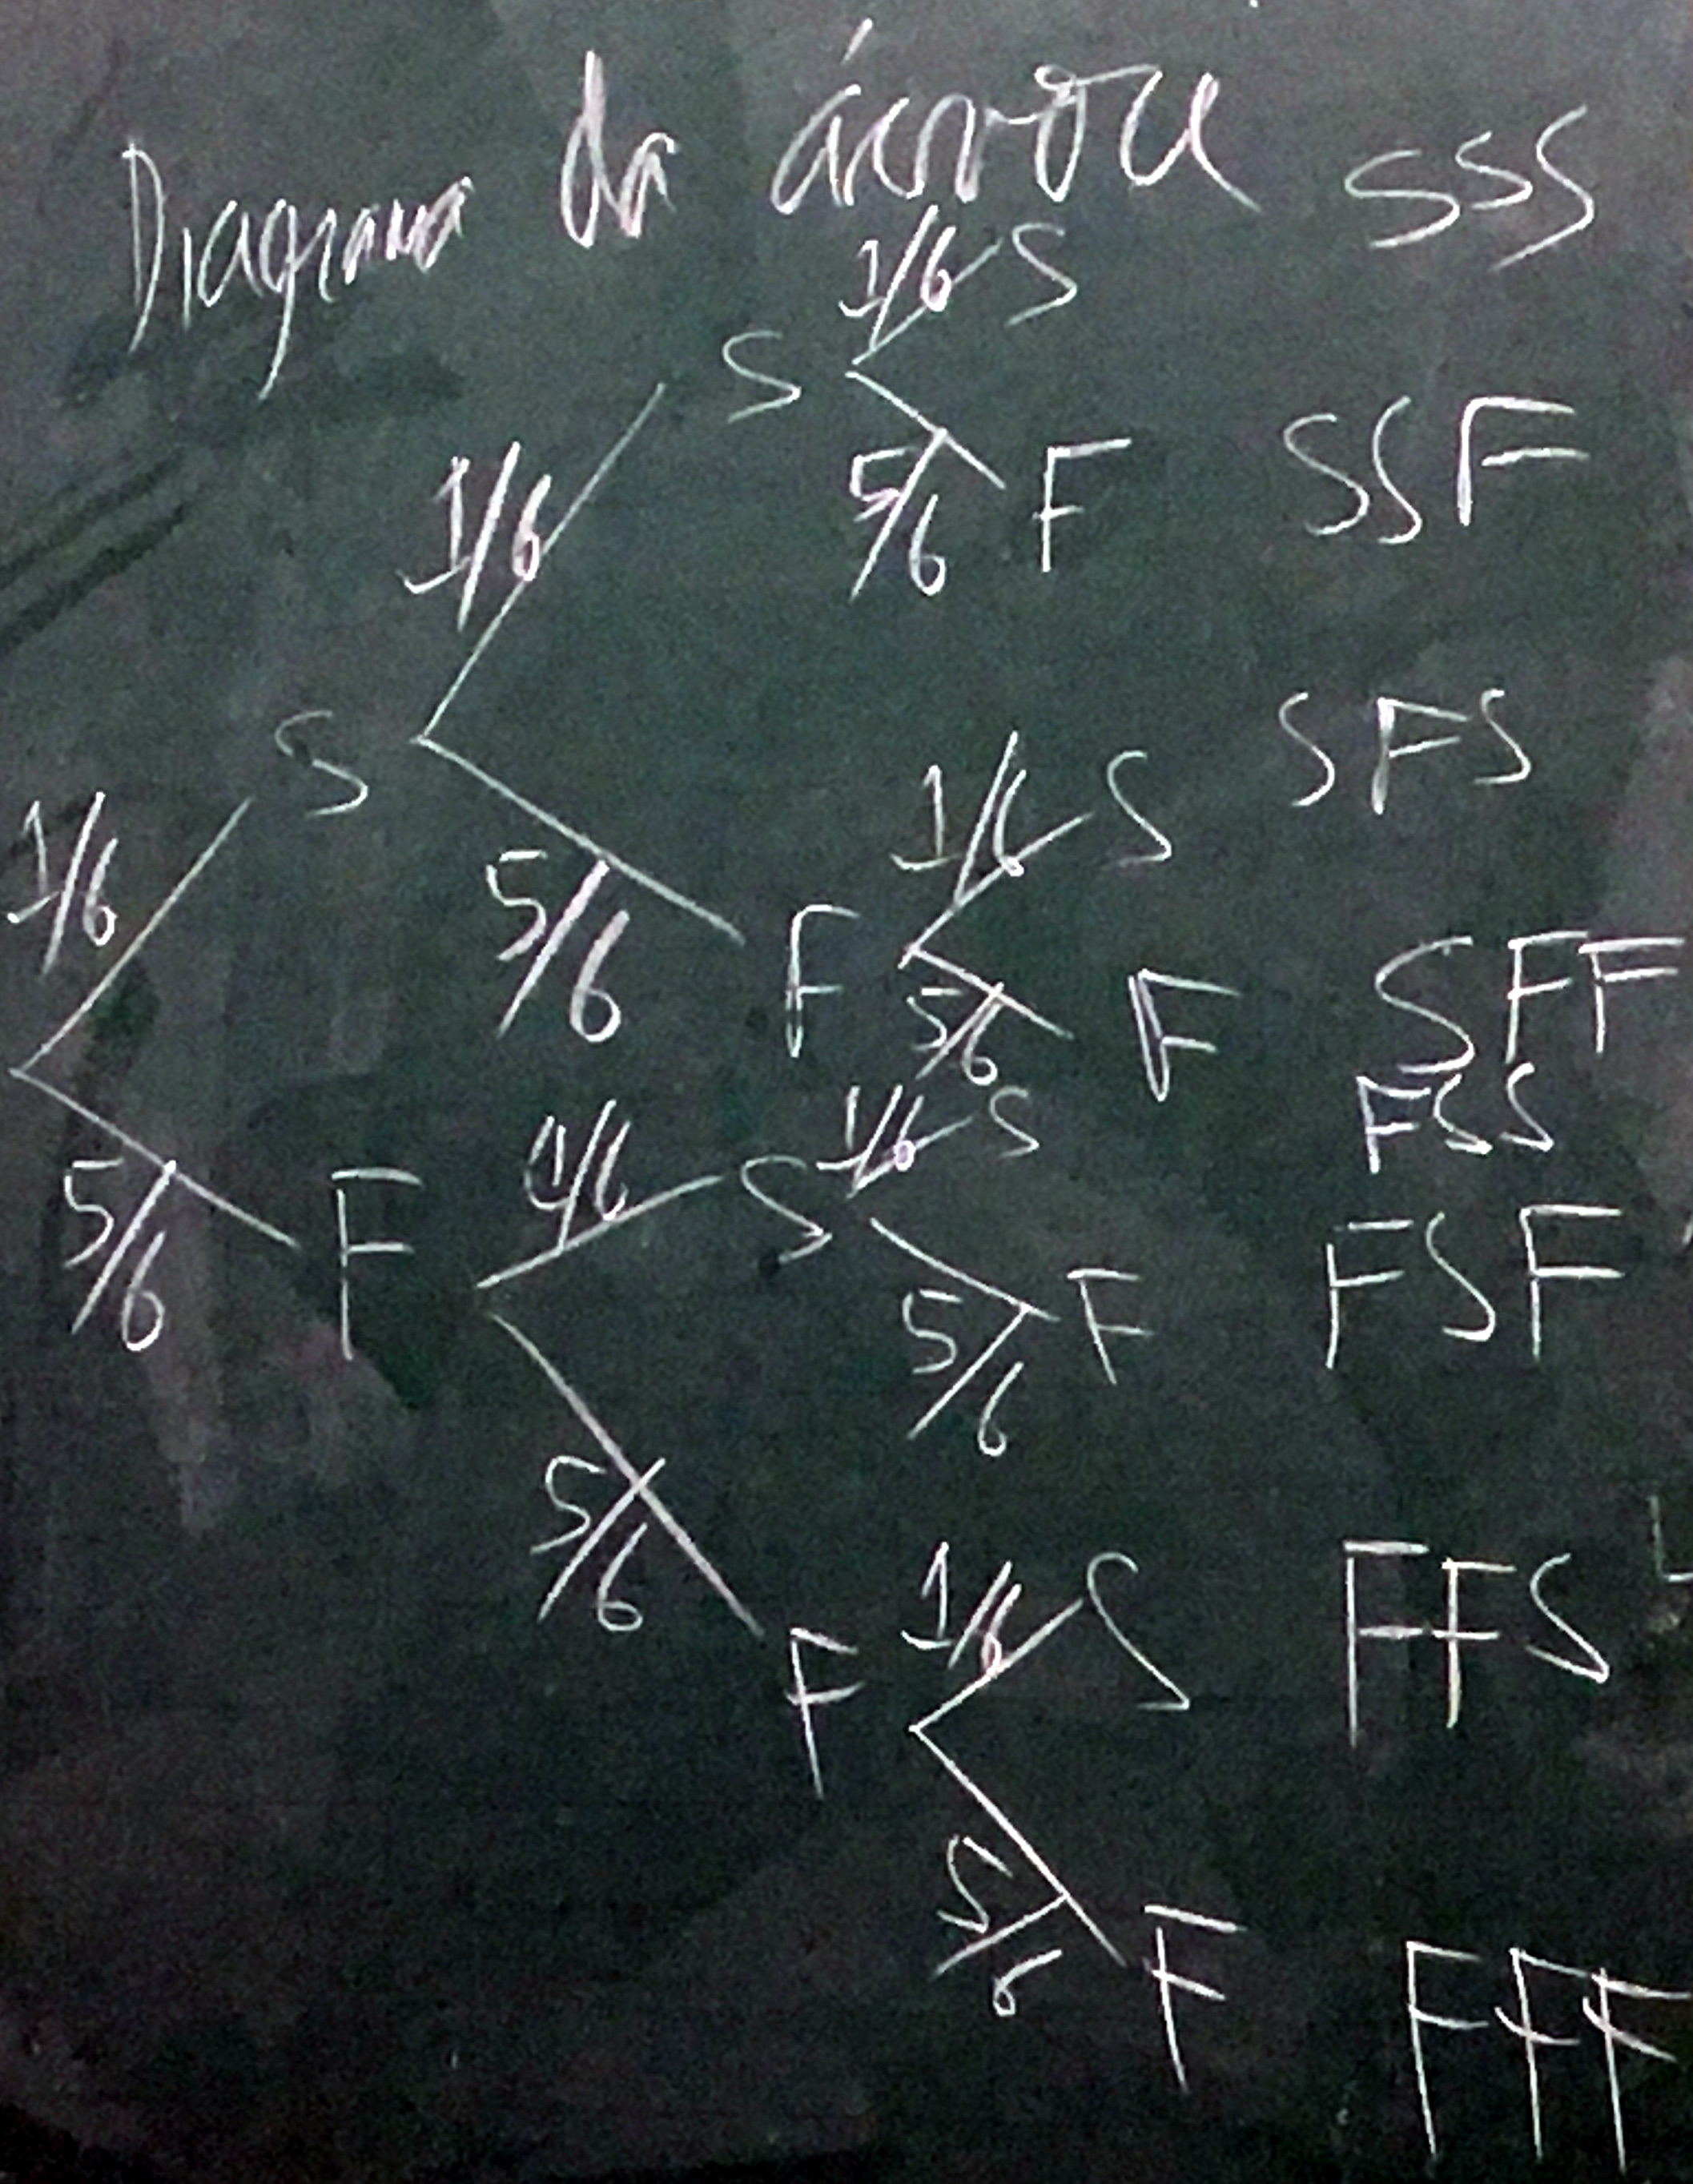
\includegraphics[width=0.7\linewidth]{img/2019-08-02_IMG-6448}
	\end{figure}	
	
	Vamos construir a distribuição de frequências (\autoref{tab:pbinomial}).
	
	\begin{table}[h]
	\centering
	\caption{Tabela de distribuição de probabilidade de $X$}
	\label{tab:pbinomial}
	\begin{tabular}{l|l}
		\textbf{$X$} & \textbf{$P(X)$} \\ \hline \\
		$0$ & $(\frac{5}{6})^3 = 57,9\%$ \\ \\
		$1$ & $3 \times (\frac{5}{6}) \times (\frac{1}{6}) = 34,7\%$ \\ \\
		$2$ & $3 \times (\frac{5}{6}) \times (\frac{1}{6})^2 = 6,9\%$ \\ \\
		$3$ & $(\frac{1}{6})^3 = 0,5\%$	\end{tabular}
	\end{table}

	\notagrande{Lembrando que a soma das probabilidades na distribuição precisa dar 100\%}
	
	A tabela nada mais é do que $X = Bin\left(3,\dfrac{1}{6}\right)$.

	\subsubsection{Proposição}
	
	Seja $X=Bin(n,p)$ então $p(X=S)=C_{n,s} \cdot p^2 (1-p)^{n-s}$.
	
	\subsubsection{Exemplo}
	
	Um vendedor faz uma venda com 20\% de probabilidade de sucesso. Qual a probabilidade de fazer duas ou mais vendas em um dia que fez dez visitas?
	
	O experimento é realizar as $10$ visitas.
	
	$S =$ vender
	
	$F =$ não vender
	
	$X =$ quantidade de vendas em $10$ visitas
	
	$X = Bin(10,20\%)$
	
	Queremos:
	
	$p(X \geq 2) = ?$
	
	Temos: 
	
	$p(X=0) = C_{10,0} (20\%)^0 \cdot (80\%)^{10} = 1 \cdot (80\%)^{10} = 10,7\%$
	
	$p(X=1)=C_{10,1} (20\%)^1 \cdot (80\%)^9 = 26,8\%$
	
	Logo: 
	
	$p(X \geq 2) = 100\% - 10,7\% - 20,8\% = 62,5\%$.
	
	\subsection{Esperança, variância e desvio padrão}
	
	Proposição:
	
	Seja $X = Bin(n,p)$ então:
	
	$E(X) = np$
	
	$Var(X) = np(1\times p)$
	
	$DP(X) = \sqrt{np(1-p)}$
	
	\subsubsection{Exemplo}
	
	Vendedor.
	
	$p(S) = 20\%, 10$ visitas
	
	$X =$ quantidade de visitas
	
	Solução:
	
	$X = Bin(10,20\%)$
	
	$E(X) = 10 \times 20\% = 2$
	
	$Var(X) = 10 \times 20\% \times 80\% = 1,6$
	
	$DP(X) = \sqrt{1,6} = 1,3$
	
	\aula{Início da aula de 06/08/2019}
	
	\section{Distribuição normal}
	
	Ementa:
	
	\begin{itemize}
		\item Distribuição contínua uniforme
		\item Distribuição discreta $\times$ distribuição contínua
		\item Distribuição normal padrão
		\item Distribuição normal
		\item Teorema do limite central
	\end{itemize}

	\subsection{Distribuição uniforme}
	
	Função $f(X) =$ função densidade de probabilidade.
	
	A probabilidade está associada à área, logo, $probabilidade\leftrightarrow area$. Temos:
	
	\begin{equation*}
		p(r \leq X \leq r) = \dfrac{r - s}{b -a}
	\end{equation*}
	
	\begin{equation*}
		p(a \leq X \leq b) = 100\% = (b-a) \times \dfrac{1}{b-a}
	\end{equation*} 
	
	A probabilidade de todos os casos definidos deve ser de $100\%$.
	
	\subsubsection{Exemplo}
	
	\noindent \textbf{Compra de apartamento:} corretor recomenda ofertar entre $250.000$ e $300.000$. Qual a probabilidade de o vendedor aceitar $280.000$?
	
	$P(250 \leq X \leq 280) = \dfrac{280 - 250}{300 - 250} = 60\%$
	
	\subsection{Discreta vs. contínua}
	
	\begin{table}[h]
		\centering
		\caption{Distribuição discreta $\times$ distribuição contínua}
		\label{tab:pbinomialc}
		\begin{tabular}{l|l|l|l}
			\textbf{$X$ contínua} & \textbf{$P$ discreta} & \textbf{$X$ contínua} & \textbf{$P$ contínua} \\ \hline
			$X_1$ & $P_1$ & $X_1$ & $0$ \\
			$X_2$ & $P_2$ & $X_2$ & $0$ \\
			$X_3$ & $P_3$ & $X_3$ & $0$
		\end{tabular}
	\end{table}

	\begin{itemize}
		\item Discreta
		\begin{itemize}
			\item $P(X=X_i) \neq 0$
			\item Descrição: tabela de distribuição de probabilidades (em valores e probabilidades)
		\end{itemize}
		\item Contínua
		\begin{itemize}
			\item $P(X=X_i) = 0$
			\item Descrição: tabela de distribuição de intervalos e probabilidades
		\end{itemize}
	\end{itemize}
	
	\section{Distribuição normal padrão}
	
	Notação: distribuição normal padrão com média $o$ e variância $1$:
	
	\begin{equation*}
		N(0,1)
	\end{equation*}
	
	Proposição:
	
	\begin{equation*}
	Z = N(0,1)
	\end{equation*}
	
	\begin{enumerate}
		\item $P(Z \leq Z_1) = P(Z \geq -Z_1)$
		\item $P(Z \geq Z_1) = 100\% - P(Z \leq Z_1)$
		\item $P(Z_1 \leq Z \leq Z_2) = P(Z \ leq Z_2) = P(Z \ leq Z_1)$
	\end{enumerate}
	
	\subsection{Uso da tabela da normal padrão}
	
	\begin{equation*}
		P(Z < z)
	\end{equation*}
	
	\subsubsection{Exemplo}
	
	Usar tabela em \url{https://www.ime.unicamp.br/~hlachos/Tabela_Normal.pdf}.
	
	\begin{enumerate}[label=\alph*.]
		\item $p(Z \leq 1,2)$ \\
		$p(Z \leq 1,2) = p(Z \leq 1,20) = 88,49\%$
		\item $p(Z \geq 2,33)$ \\ $p(Z \geq 2,33) = 100\% - p(Z \leq 2,33) = 100\% - 99,01\% = 0,99\%$
		\item $p(1,2 \leq Z \leq 2,33)$ \\
		$p(1,2 \leq Z \leq 2,33) = P(Z \leq 2,33) - P(Z \leq 1,2) = 99,01\% - 88,49\% - 10,52\%$
		\item $p(-1 \leq Z \leq 1)$ \\
		$p(-1 \leq Z \leq 1) = p(Z \leq 1) - p(Z \leq -1)$ \\
		Temos: $p(Z \leq 1) = 84,13\%$ e $p(Z \leq -1) = 100-84,13\% = 15,87\%$ \\
		$p(-1 \leq Z \leq -1) = 84,13\% - 15,87\% = 68,26\%$
		\item $p(-1,96 \leq Z \leq 1,96)$ \\
		$p(Z \leq 1,96) - p(Z \leq -1,96) = 97,50\% - (100\% - 97,50\%) = 95\%$
	\end{enumerate}

	À alínea (c) significa que a probabilidade de ocorrer um valor que esteja 1 desvio padrão da média é de $68,26\%$.
	
	\subsection{Distribuição normal}
	
	Proposição:
	
	Se $X = N(\mu, \sigma^2)$ = normal com média $\mu$ e variância $\sigma^2$, então:
	
	\begin{enumerate}
		\item $Z = \dfrac{Z-\mu}{\sigma}$ é uma $N(0,1)$
		\item $p(X \leq X_1) = p(Z \leq Z_1)$ para $Z_1 = \dfrac{X_1 - \mu}{\sigma}$
	\end{enumerate}

	\subsubsection{Exemplo}
	
	Um pneu roda em km $N\left(58000, (8000)^2\right)$.
	
	\begin{enumerate}[label=\alph*.]
		\item $p(X \leq 50000)$ \\
		$= p\left(Z \leq \dfrac{50000 - 58000}{8000}\right)$ \\
		$= p(Z \leq -1) = 100\% - 84,13\% = 15,87\%$
		\item $p(X \geq 70000)$ \\
		$=100\% - p(X \leq 70000)$ \\
		$=100\% - p\left( Z \leq \dfrac{70000 - 58000}{8000} \right)$ \\
		$= 100\% - p(Z \leq 1,5) = 100\% - 93,22\% = 6,68\%$ \\ \\
		$p(50000 \leq X \leq 70000) = p(X \leq 70000) - p(X \leq 50000)$ \\
		$= 93,32\% - 15,87\% = 77,45\%$4
		\item Garantia mínima a oferecer um custo de $2\%$ \\
		$p(X \leq X_*) = 2\%$ \\
		$p(X \leq X_*) = p(Z \leq Z_*)$ \\
		\\
		Vamos pegar o simétrico dele: \\
		\\
		$p(Z \leq -Z_*) = 98\%$ \\
		\\
		Temos: \\
		\\
		$-Z_* = 2,05$ logo $Z_* = -2,05$ \\
		\\
		Então: \\
		\\
		$Z_* = \dfrac{X_* - \mu}{\sigma}$ \\
		$X_* = \mu + \sigma Z_* = 58000 - 2,05 \times 8000 = 91600$
	\end{enumerate}
	
	\subsection{Teorema do limite central}
	
	Sejam $X_1$, $X_2$, $\dots$ distribuições com média $\mu$ e desvio padrão $\sigma$ e independentes:
	
	\begin{enumerate}
		\item $X_1 + X_2 + \dots +X_n$ é $N(n\mu, n\sigma^2)$
		\item $\dfrac{X_1 + X_2 + \dots + X_n}{n}$ é $N\left( \mu,\dfrac{\sigma^2}{n} \right)$
	\end{enumerate}
	
	% ----------------------------------------------------------
	
	
	%
	
	\listoftodos[Lista de anotações]
	\addcontentsline{toc}{section}{Lista de anotações}
		
	\bibliography{fontes.bib}
	\addcontentsline{toc}{section}{Referências}

\end{document}


